\section{管式与釜式反应器反应体积的比较}


\begin{frame}
    \frametitle{管式与釜式反应器反应体积的比较}

    在原料处理量及组成、反应温度以及最终转化率均相同的情况下，比较管式与釜式反应器所需的反应体积。
    \begin{figure}
        \centering
        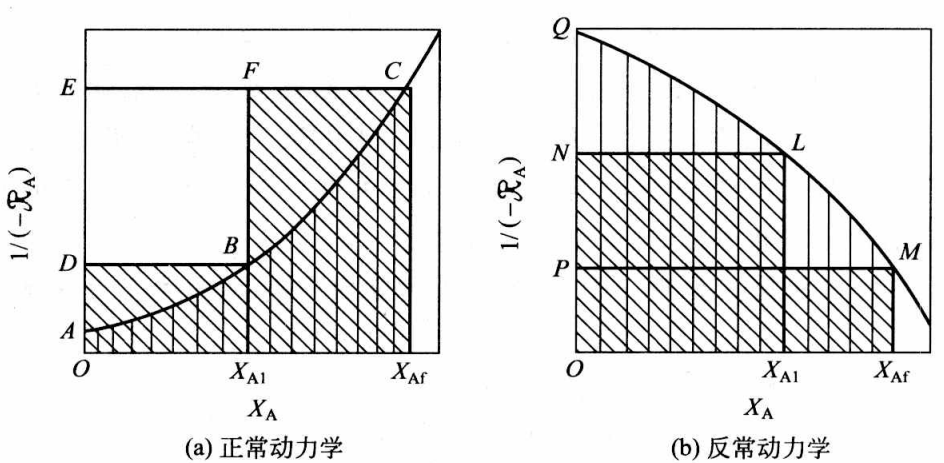
\includegraphics[width=.78\linewidth]{figs/fig4.3.png}
    \end{figure}

\end{frame}


\begin{frame}
    \frametitle{管式与釜式反应器反应体积的比较}

    一种特殊情况：反应速率与转化率的关系存在一极大值。

    ~\\
    \begin{minipage}{.48\linewidth}
        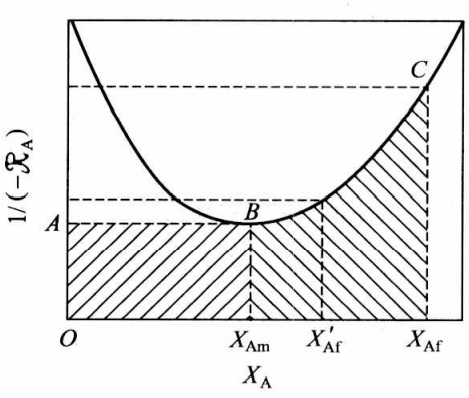
\includegraphics[width=\linewidth]{figs/fig4.4.png}
    \end{minipage}\hfill
    \begin{minipage}{.48\linewidth}
        \begin{itemize}
            \item[\bullet] 若最终转化率小于$X_\mathrm{Am}$，$V_\text{管}>V_\text{釜}$
            \item[\bullet] 若最终转化率大于$X_\mathrm{Am}$，
            
            $V_\text{管}$可能大于也可能小于$V_\text{釜}$
        \end{itemize}
        最终转化率大于$X_\mathrm{Am}$情况下，最好的办法是采用两个反应器串联，先用釜式反应器使转化率达到$X_\mathrm{Am}$，再用管式反应器。
    \end{minipage}

\end{frame}


\begin{frame}
    \frametitle{管式与釜式反应器收率的比较}
    \begin{figure}
        \centering
        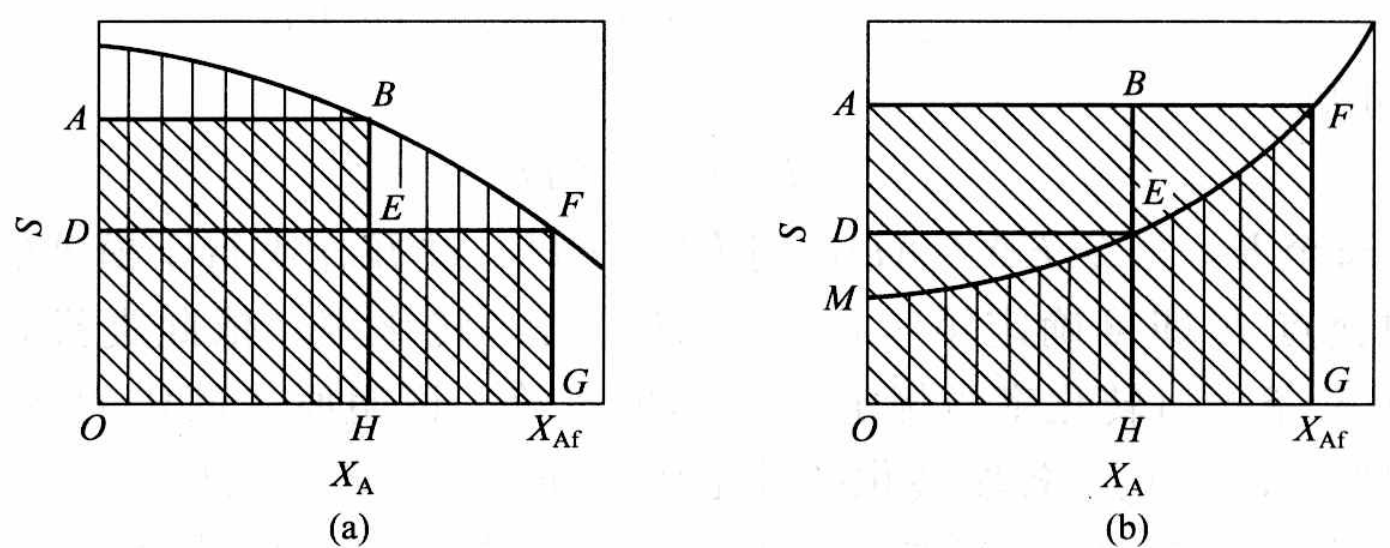
\includegraphics[width=.9\linewidth]{figs/fig3.9.png}
    \end{figure}
    间歇釜式反应器的性能与等容下的管式反应器相同。

    (a)管式反应器的最终收率大于连续釜式反应器。(b)反之。

\end{frame}


\begin{frame}
    \frametitle{管式反应器的加料方式}

    \begin{minipage}{0.42\linewidth}
        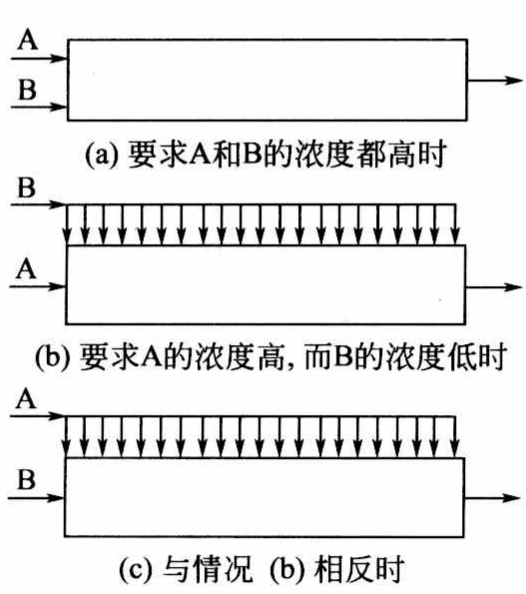
\includegraphics[width=\linewidth]{figs/fig4.5.png}
    \end{minipage}\hfill
    \begin{minipage}{0.56\linewidth}
        根据对反应物浓度的不同要求，可以对管式反应器采用不同的加料方式。
        \begin{itemize}
            \item[(a)] 当要求A和B的浓度都高时，可将两者同时在反应器的一端加入
            \item[(b)] 如要求A的浓度高，而B的浓度低，除了可以使进料中A大量过剩外，也可将A全部由反应器一端加入，而B则沿反应器的轴向分段加入。
            \item[(c)] 要求A的浓度低，B的浓度高时按图c加料。
        \end{itemize}
    \end{minipage}

\end{frame}


\begin{frame}[t]
    \frametitle{}

    \begin{example}
        拟设计一等温反应器进行下列液相反应
        \[
            \ch{A + B -> R} \qquad r_\mathrm{R}=k_1c_\mathrm{A}c_\mathrm{B}
        \]
        \[
            \ch{2 A -> S} \qquad r_\mathrm{S} = k_2 c_\mathrm{A}^2
        \]
        目的产物是R，且R与B极难分离。试问

        (1) 在原料配比上有何要求？

        (2) 若采用活塞流反应器，应采用什么样的加料方式？

        (3) 如用半间歇反应器，又应用什么样的加料方式？
    \end{example}

\end{frame}


\begin{frame}[t]
    \frametitle{}

    \begin{question}
        习题4.14

        习题4.18
    \end{question}

\end{frame}


